% Global document settings
\documentclass[10pt]{article}

% Packages
\usepackage{tgtermes}
\usepackage{graphicx}
\usepackage{natbib}
\usepackage{authblk}
\usepackage{array}
\usepackage{colortbl}
\usepackage{tocloft}
\usepackage{xcolor}
\usepackage{siunitx}
\usepackage{setspace}
\usepackage{listings}
\usepackage{caption}
\usepackage[T1]{fontenc}
\usepackage[nottoc]{tocbibind}
\usepackage[breaklinks]{hyperref}
\usepackage[font=small,skip=7pt]{caption}

% Custom colours
\definecolor{codegreen}{rgb}{0,0.6,0}
\definecolor{codegray}{rgb}{0.5,0.5,0.5}
\definecolor{codepurple}{rgb}{0.58,0,0.82}
\definecolor{backcolour}{rgb}{0.95,0.95,0.92}

% Listing styles
\lstdefinestyle{mystyle}{
  backgroundcolor=\color{backcolour},
  commentstyle=\color{codegreen},
  keywordstyle=\color{purple},
  numberstyle=\tiny\color{codegray},
  stringstyle=\color{codepurple},
  basicstyle=\ttfamily\footnotesize,
  breakatwhitespace=false,
  breaklines=true,
  captionpos=b,
  keepspaces=true,
  numbers=left,
  numbersep=5pt,
  showspaces=false,
  showstringspaces=true,
  showtabs=false,
  tabsize=2
  }
  \lstset{style=mystyle}

  % Custom commands
  \renewcommand{\bibname}{References} % Change bibliography title
  \renewcommand\cftsecafterpnum{\vskip8pt}
  \renewcommand{\lstlistlistingname}{List of \lstlistingname s}
  \renewcommand{\bibsection}{\section*{Bibliography}}
  \renewcommand{\contentsname}{Table of Contents}
  \renewcommand{\bibsection}{\section{\bibname}}
  \renewcommand{\cftsecleader}{\cftdotfill{\cftdotsep}}

  % Custom settings
  \captionsetup{justification=centering}
  \PassOptionsToPackage{hyphens}{url}
  \urlstyle{same}
  \def\Urlmuskip{0mu}
  \def\UrlBreaks{\do\/\do-}
  \hypersetup{
    colorlinks = true,
    urlcolor = blue,
    linkcolor = black,
    citecolor = black,
  breaklinks=true,
  pdfpagemode=UseOutlines,
  bookmarksopen=true,
  bookmarksopenlevel=2,
  bookmarksnumbered=true
  }

  \title{\textbf{Flicking the Switch: } \\ Optogenetics and the Interplay of Direct and \\ Indirect Pathways in Motor Control}
  \author[ ]{Daniel Burger}
  \affil[ ]{\textbf{King’s College London}}
  \affil[ ]{\href{mailto:public@danielburger.online}{public@danielburger.online}}
  \date{\textit{8. August 2023}}

\begin{document}
\pagenumbering{roman}
\counterwithin{lstlisting}{section}
\counterwithin{figure}{section}
\counterwithin{table}{section}

\maketitle
\thispagestyle{empty}

% Double spacing for feedback
% \doublespacing

\begin{sloppypar} % For better line breaks
  \begin{abstract}
    This essay comprehensively synthesises the current understanding of the basal ganglia’s direct and indirect pathways. It critically examines the traditional dichotomous model and explores recent evidence suggesting a more nuanced, dynamic interaction between these pathways across various functions, including motor control, decision-making, reward processing, and motor learning. By focusing on key studies employing optogenetics, the essay offers insights into these pathways’ concurrent activation and divergence during action initiation and execution, thereby challenging the traditional binary view.

    The essay also discusses the implications of alterations in these pathways for the manifestation of Parkinson’s disease symptoms and the potential for therapeutic interventions. It emphasises the significant contributions of optogenetics to our knowledge of these pathways while acknowledging its limitations. Despite the advancements in our understanding of basal ganglia circuit dynamics, the essay highlights remaining open questions regarding the precise mechanisms coordinating pathway interactions during action selection and learning, underscoring the need for continued research in this fascinating field.
  \end{abstract}
  \pagebreak

  \pagenumbering{Roman}
  \tableofcontents
  \pagebreak

  \listoffigures
  \pagebreak

  % \listoftables
  % \pagebreak

  % Back to normal numbering
  \pagenumbering{arabic}

  \section{Introduction}
  \label{sec:introduction}

  Parkinson’s disease, a prevalent neurodegenerative disorder, primarily affects the basal ganglia, a group of subcortical nuclei in the brain. These nuclei, which include key structures such as the striatum, globus pallidus, subthalamic nucleus, and substantia nigra, play crucial roles in motor control, decision-making, and reward processing \citep{zhang_oculomotor_2018, ojagbemi_neuropsychiatric_2013}.

  The motor symptoms of Parkinson’s disease, such as rigidity, tremors, and bradykinesia, are often attributed to the degeneration of dopaminergic neurons in the substantia nigra, a critical component of the basal ganglia \citep{abedini_cooccurrence_2015}. The resultant disruption in the balance and functioning of the basal ganglia’s direct and indirect pathways, which are primarily composed of medium spiny neurons (MSNs), has significant implications for motor control \citep{abedini_cooccurrence_2015,ojagbemi_neuropsychiatric_2013}.

  Traditionally, the direct and indirect pathways of the basal ganglia are thought to function antagonistically: the direct pathway facilitates movement, while the indirect pathway inhibits it \citep{isett_indirect_2022}. However, recent studies have challenged this dichotomous model, suggesting a more complex interaction between these pathways. For instance, these pathways may display potential concurrent activation and divergence in certain motor actions, adding complexity to our understanding of their roles in voluntary movement control \citep{perez_striatal_2017}.

  \begin{figure}[ht]
    \centering
    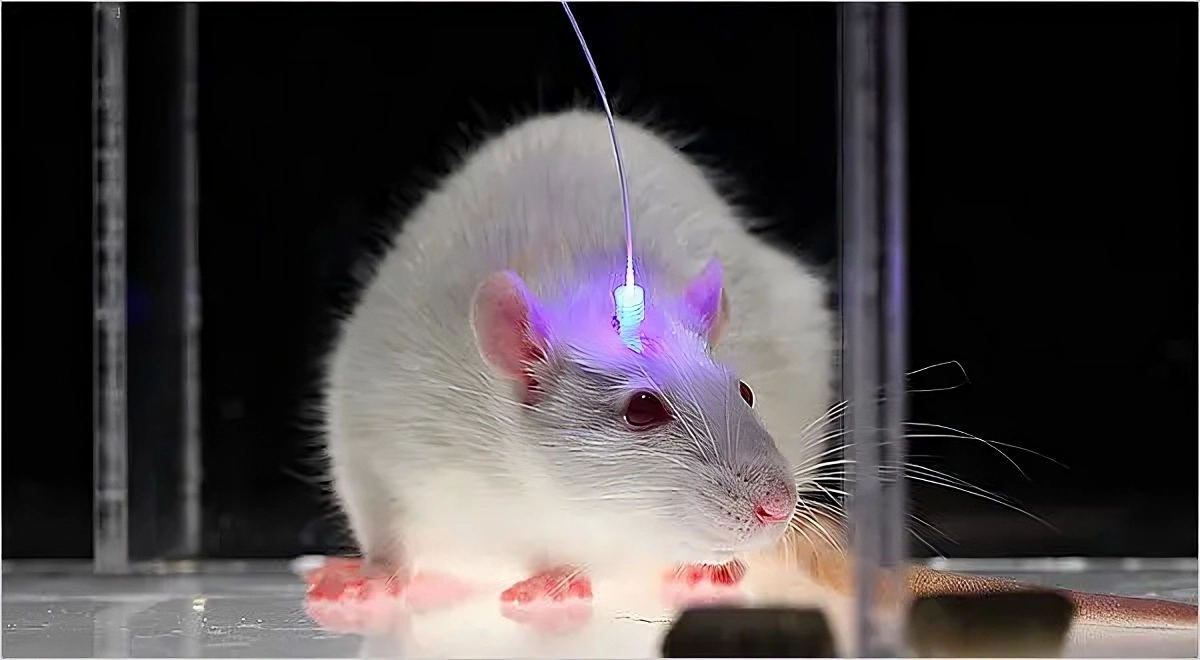
\includegraphics[width=\textwidth]{figures/optogenetics.png}
    \caption[A rat equipped with an optogenetic implant]{\textbf{A rat equipped with an optogenetic implant.} The probe seen here, part of an optogenetic implant, can measure or manipulate neuronal signals, offering precise control over specific neural pathways. Image credit: The New York Times \citep{belluck_risky_2016}.}
    \label{fig:optogenetics}
  \end{figure}

  The advent of optogenetics, a technique that allows precise manipulation of specific neurons using light \citep{deisseroth_next-generation_2006}, has significantly advanced our understanding of the basal ganglia pathways. Optogenetics involves the genetic modification of neurons to express light-sensitive proteins known as opsins. These opsins can be activated or inhibited by exposure to certain wavelengths of light via an implanted device, as depicted in \autoref{fig:optogenetics}. Notably, \cite{kravitz_regulation_2010} used optogenetics to activate direct and indirect pathway MSNs selectively, providing key insights into their functions and contribution to the traditional model of the basal ganglia.

  Continuing developments in optogenetic investigations have proposed that these pathways may function bidirectionally, with the specific function depending on the context or the motor behaviour being executed \citep{yttri_opponent_2016}. This revelation, along with recent studies expanding our understanding of these pathways’ roles in reward-based learning, motor learning, and movement velocity regulation \citep{hilt_evidence_2016, wang_direct_2015}, underscores the complexity of basal ganglia pathways.

  This essay synthesises our current knowledge of the basal ganglia pathways’ role in motor control and decision-making, focusing on the insights provided by optogenetic studies. The following section explores significant research that has challenged the traditional model of these pathways.

  \section{Challenging the Traditional Model}
  \label{sec:challenging-the-traditional-model}

  The traditional model of the basal ganglia’s direct and indirect pathways has been significantly advanced by the pivotal work of \cite{cui_concurrent_2013}. They proposed a more dynamic interaction between the direct and indirect pathways during action selection, a significant departure from the conventional understanding.

  In their study, \citeauthor{cui_concurrent_2013} employed optogenetic techniques to explore this interaction. They focused on the MSNs in the dorsomedial striatum of mice, the origin points of the direct and indirect pathways, and manipulated neuronal activity precisely to study its effects on action selection.

  \begin{figure}[ht]
    \centering
    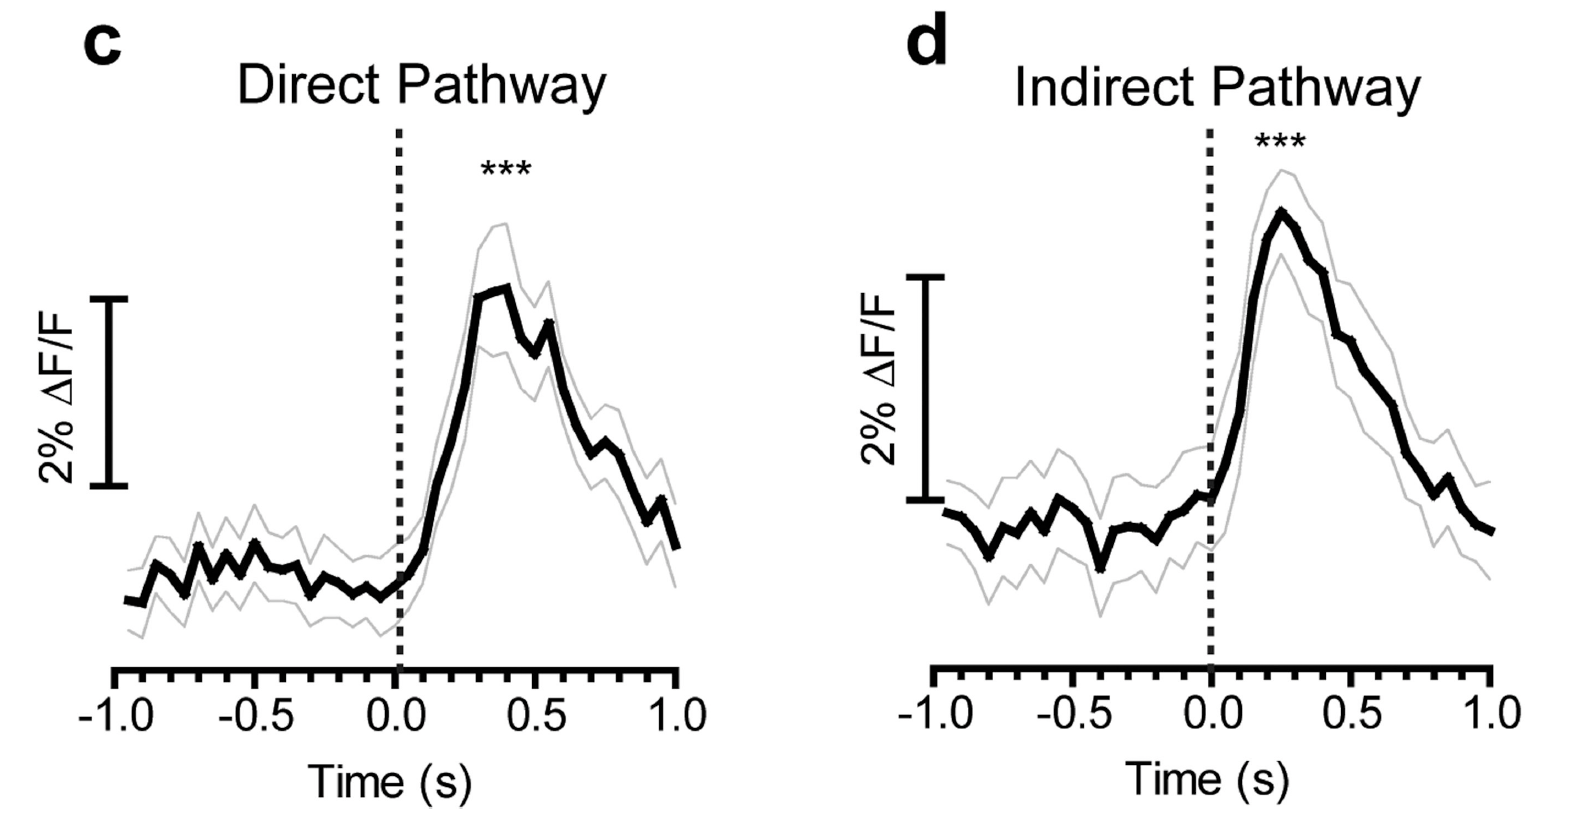
\includegraphics[width=\textwidth]{figures/direct-indirect-activation.png}
    \caption[Concurrent activation of direct and indirect pathways during action initiation]{\textbf{Concurrent activation of direct and indirect pathways during action initiation.} This figure, based on data from \cite{cui_concurrent_2013}’s study, demonstrates the concurrent activation of direct-pathway medium spiny neurons (dMSNs) and indirect-pathway medium spiny neurons (iMSNs) at the start of a lever-pressing session. The fluorescence traces indicate increased activity for both dMSNs and iMSNs at the session start, challenging the classical model’s assertion of opposing activation of these pathways.}
    \label{fig:pathway-activation}
  \end{figure}

  \citeauthor{cui_concurrent_2013}’s key revelation was the concurrent activation of both the direct and indirect pathways during the initiation of a movement. As illustrated in \autoref{fig:pathway-activation}, both types of neurons increased their firing rates at the start of a lever-pressing session, contradicting the conventional model’s assertion of opposing activation of these pathways.

  Moreover, they observed that the activity of iMSNs and dMSNs varied during the actual movement execution. While dMSN activity remained high, iMSN activity decreased, suggesting that although both pathways are involved in action initiation, their roles may differ during action execution.

  Interestingly, both types of neurons were inactive when the rats were not moving, further challenging the conventional understanding and suggesting a more nuanced interplay between the direct and indirect pathways. This complexity was underscored in \cite{guillaumin_experimental_2021}’s study, which revealed the involvement of both pathways in reward-based learning, a process where an individual learns to perform certain actions based on the reward they receive.

  \section{Complementary and Contrasting Studies}
  \label{sec:complementary-and-contrasting-studies}

  Building on this understanding, several studies have furthered our knowledge of the basal ganglia pathways, each adding a unique perspective to the findings of \cite{cui_concurrent_2013}.

  In a similar vein to \citeauthor{cui_concurrent_2013}, \cite{yttri_opponent_2016} used optogenetic stimulation to explore the role of these pathways in the bidirectional control of movement velocity. They found that both pathways can regulate movement velocity and speed, suggesting a capacity for cooperative action that extends beyond the concurrent activation observed by \citeauthor{cui_concurrent_2013} during action initiation.

  \cite{guillaumin_experimental_2021} took a different approach, investigating the role of these pathways in reward-based learning. They showed that direct pathway activation enhanced reward-seeking behaviour while indirect pathway activation suppressed it. This indicates that both pathways also participate in reward processing. This cognitive function shares neural circuits with motor control, further reinforcing the complexity and versatility of these pathways beyond the context of movement initiation.

  \cite{hilt_evidence_2016} focused on motor learning, finding that activation of the direct pathway facilitated motor learning, while activation of the indirect pathway impaired it. Although this may seem to contrast with \cite{cui_concurrent_2013}’s findings, it may reflect the different neural dynamics and populations engaged in motor learning and action initiation. This highlights the diverse roles of these pathways in various aspects of motor control.

  Lastly, \cite{wang_direct_2015} explored how these pathways regulate movement speed control. They found that the direct pathway facilitated an increase in speed, while the indirect pathway led to a decrease.

  \newpage

  This observation supports \cite{cui_concurrent_2013}’s findings of the concurrent activation of both pathways during action initiation, suggesting that these pathways might work together to fine-tune motor parameters such as speed during action execution.

  In light of these studies, it is evident that the diverse roles of the direct and indirect pathways in the basal ganglia extend from motor control to reward processing, enriching our understanding of their complex dynamics and interactions.

  \section{Optogenetics in Decoding Neural Pathways}
  \label{sec:the-role-of-optogenetics-in-neural-pathways}

  Optogenetics, a revolutionary tool in neuroscience, has played a transformative role in decoding the intricate dynamics of neural pathways. It employs light-sensitive proteins known as opsins to control and observe specific neurons’ activity in living tissue with great precision. This technique operates based on genetic modifications, allowing opsins to be selectively expressed in specific types of neurons through viral vectors or transgenic animals, where opsins are introduced under the control of neuron-specific promoters \citep{deisseroth_next-generation_2006}.

  Optogenetics has been instrumental in the studies discussed so far, enabling researchers to investigate the dynamic interactions between the direct and indirect pathways of the basal ganglia. For instance, \cite{yttri_opponent_2016} applied optogenetics to explore the complexity of how these pathways can bidirectionally regulate movement velocity, thereby extending our understanding beyond the conventional model of antagonistic pathway function.

  \cite{guillaumin_experimental_2021} employed optogenetics to explore the motivational aspects of behaviour, providing insights into the participation of both pathways in reward processing. This shows how optogenetics can broaden our perspective, highlighting the application of these pathways beyond the context of movement initiation.

  Despite the valuable insights optogenetics provides, it is important to acknowledge its limitations. The necessity for genetic modifications can pose challenges, especially in non-model organisms, and delivering light to deep brain structures can be technically challenging. Moreover, neurons’ artificial activation or inhibition may not fully represent the complex dynamics of natural neuronal activity.

  Nevertheless, optogenetics has undeniably revolutionised neuroscience, providing novel insights into the functioning of neural pathways, including the direct and indirect pathways of the basal ganglia. As our understanding and application of optogenetics continue to evolve, we can expect it to shed more light on the brain’s complex workings and potentially contribute to developing treatments for neurological disorders.

  \section{Conclusion}
  \label{sec:conclusion}

  While we have made significant strides in understanding the basal ganglia’s direct and indirect pathways, key questions remain. Future research needs to elucidate the precise mechanisms coordinating pathway interactions during action selection and learning. It is also crucial to investigate how these pathways interact with other neural circuits in the brain to orchestrate complex behaviours.

  The continuing evolution of optogenetic techniques offers exciting possibilities for future research. As these techniques become more refined, they will enable more precise and detailed investigations of neural circuit dynamics. This could lead to a deeper understanding of the basal ganglia’s roles in health and disease and potentially contribute to new therapeutic strategies for neurological disorders such as Parkinson’s.

  In summary, our understanding of the basal ganglia’s direct and indirect pathways has significantly advanced, moving beyond the traditional dichotomous model to a more nuanced view of these pathways as dynamic, cooperative entities. This perspective shift has been driven, in large part, by the advent of optogenetic techniques, which have allowed researchers to probe neural circuit dynamics with unprecedented precision. As we look to the future, there is no doubt that our understanding of these intricate neural circuits will continue to deepen, promising exciting new insights into the brain’s complex workings.

  \pagebreak
  \singlespacing % No need for double spacing in the references
  \bibliographystyle{references/custom-apa}
  \bibliography{references/bibliography}

\end{sloppypar}
\end{document}